\renewcommand{\FileName}{nested}
% slide template
\subsection{Basic ideas}
\begin{frame}
  \frametitle{Polytomous response: Nested dichotomies}
  \begin{itemize}
    \item $m$ categories $\rightarrow (m-1)$ comparisons (logits)
	\item If these are formulated as $(m-1)$ nested dichotomies:
      \begin{itemize*}
		\item Each dichotomy can be fit using the familiar binary-response
       logistic model,
		\item the \(m - 1\) models will be statistically independent (\(G^2\) statistics will be additive)
		\item (Need some extra work to summarize these as a single, combined model)
	  \end{itemize*}
	\item This allows the slopes to differ for each logit
  \end{itemize}
\begin{center}
  \includegraphics[width=0.9\textwidth]{fig/nested2}
\end{center}
\end{frame}

\begin{frame}
\begin{center}
  \frametitle{Nested dichotomies: Examples}
  \includegraphics[width=0.9\textwidth]{fig/nested1c}
\end{center}
 
\end{frame}

\begin{frame}
  \frametitle{Example: Women's Labour-Force Participation}
Data: \emph{Social Change in Canada Project} , York ISR \citep{Fox:97}
  \begin{itemize}
	\item{\large\bfseries Response:} not working
outside the home (n=155), working part-time (n=42)  or working
full-time (n=66)
   \item Model as two nested dichotomies:
	 \begin{itemize*}
	 \item Working (n=106) vs.\ NotWorking (n=155)
	 \item Working full-time (n=66) vs.\ working part-time (n=42).
	 \end{itemize*}

	\item{\large\bfseries Predictors:}
	 \begin{itemize*}
	 \item Children? --- 1 or more minor-aged children
	 \item Husband's Income --- in \$1000s
	 \item Region of Canada (not considered here)
	 \end{itemize*}
  \end{itemize}
\end{frame}

\begin{frame}[fragile]
  \frametitle{Example: Women's Labour-Force Participation}
\begin{Input}[label=\fbox{\texttt{wlfpart.sas}},baselinestretch=0.8]
proc format;
   value labour    \sascomment{/* labour-force participation */}
      1 ='working full-time'  2 ='working part-time'
      3 ='not working';
   value kids      \sascomment{/* children in the household */}
      0 ='Children absent'  1 ='Children present';
data wlfpart;
   input case labour husinc children region;
   working = labour < 3;
   if working then
      fulltime = (labour = 1);
datalines;
  1  3  15  1  3
  2  3  13  1  3
  3  3  45  1  3
  4  3  23  1  3
  5  3  19  1  3
  6  3   7  1  3
  7  3  15  1  3
  8  1   7  1  3
  9  3  15  1  3
  ... \sasemph{more data lines} ...
\end{Input}
\end{frame}

\begin{frame}[fragile]
  \frametitle{Example: Women's Labour-Force Participation}
First, try proportional odds model for \texttt{labour}

\begin{Input}[fontsize=\small]
proc logistic data=wlfpart;
   model \sasemph{labour}  = husinc children;
   title2 'Proportional Odds Model: Fulltime/Parttime/NotWorking';
\end{Input}
The score test \emph{rejects} the Proportional Odds Assumption
\begin{Output}[gobble=6]
                 Score Test for the Proportional Odds Assumption
 
                       Chi-Square       DF     Pr > ChiSq
                          18.5638        2         \sasemph{<.0001}
\end{Output}
This indicates that the slopes differ for at least one of \texttt{husinc}
and \texttt{children}.

\textbf{Note}: The score test is known to be overly sensitive. 
Use a more stringent $\alpha$ to reject.
\end{frame}

\begin{frame}[fragile]
Fit separate models for each of \texttt{working} and \texttt{fulltime}:
\begin{Input}
proc logistic data=wlfpart nosimple descending;
   model \sasemph{working} = husinc children ;
   output out=resultw p=predict xbeta=logit;
   title2 'Nested Dichotomies';

proc logistic data=wlfpart nosimple descending;
   model \sasemph{fulltime} = husinc children ;
   output out=resultf p=predict xbeta=logit;
\end{Input}
\begin{itemize*}
  \item \texttt{descending} option used to model the $\Pr (Y=1)$ -- working, or fulltime
  \item \texttt{output} statements $\rightarrow$ datasets for plotting
  \item Join for plotting:
\end{itemize*}
\begin{Input}[numbers=none]
data both;
   set resultsw resultsf;
   ...
\end{Input}
  
\end{frame}

\begin{frame}[fragile]
Output for WORKING dichotomy:
\begin{Output}[gobble=3,fontsize=\footnotesize,baselinestretch=0.8]
                    Analysis of Maximum Likelihood Estimates

               Parameter Standard    Wald       Pr >        Odds
   Variable DF  Estimate   Error  Chi-Square Chi-Square    Ratio

   INTERCPT 1     1.3358   0.3838    12.1165     0.0005     .
   HUSINC   1    -0.0423   0.0198     4.5751     0.0324    0.959
   CHILDREN 1    -1.5756   0.2923    29.0651     0.0001    0.207
\end{Output}

Output for FULLTIME dichotomy:
\begin{Output}[gobble=3,fontsize=\footnotesize,baselinestretch=0.8]
                    Analysis of Maximum Likelihood Estimates

               Parameter Standard    Wald       Pr >        Odds
   Variable DF  Estimate   Error  Chi-Square Chi-Square    Ratio

   INTERCPT 1     3.4778   0.7671    20.5537     0.0001     .
   HUSINC   1    -0.1073   0.0392     7.5063     0.0061    0.898
   CHILDREN 1    -2.6515   0.5411    24.0135     0.0001    0.071
\end{Output}
\begin{eqnarray*}
  \log \left( \frac{ \Pr ( \mbox{working} ) }
  { \Pr ( \mbox{not working} ) } \right) & = &
  1.336 - 0.042 \,  \mbox{H\$} - 1.576 \,  \mbox{kids} \\  %\label{eq:wlfnest1}
%
  \log \left( \frac{ \Pr ( \mbox{fulltime} ) }
  { \Pr ( \mbox{parttime} ) } \right) & = &
  3.478 - 0.107 \,  \mbox{H\$} - 2.652 \,  \mbox{kids}  % \label{eq:wlfnest2}
\end{eqnarray*}

\end{frame}

\begin{frame}[fragile]
  \frametitle{Combined tests for Nested Dichotomoies}
  \begin{itemize}
	\item Nested dichotomies $\rightarrow \chi^2$ tests and df for the
	separate logits are independent
	\item $\rightarrow$ add, to give tests for the full $m$-level response (\alert{manually})
  \end{itemize}
 
\begin{Output}[gobble=3,fontsize=\footnotesize,baselinestretch=0.7]
                       Global tests of BETA=0
                                                            Prob
    Test                Response         ChiSq      DF     ChiSq

    Likelihood Ratio    working        36.4184       2    <.0001
                        fulltime       39.8468       2    <.0001
                        \sasemph{ALL            76.2652       4    <.0001}
\end{Output}
Wald tests:
\begin{Output}[gobble=3,fontsize=\footnotesize,baselinestretch=0.7]
             Wald tests of maximum likelihood estimates
                                                       Prob
        Variable     Response     WaldChiSq    DF     ChiSq

        Intercept    working        12.1164    1     0.0005
                     fulltime       20.5536    1     <.0001
                     \sasemph{ALL            32.6700    2     <.0001}

        children     working        29.0650    1     <.0001
                     fulltime       24.0134    1     <.0001
                     \sasemph{ALL            53.0784    2     <.0001}

        husinc       working         4.5750    1     0.0324
                     fulltime        7.5062    1     0.0061
                     \sasemph{ALL            12.0813    2     0.0024}
\end{Output}
\end{frame}

% slide template
\subsection{Model visualization in SAS}
\begin{frame}
  \frametitle{Model visualization}
  \begin{itemize*}
	\item Join \ODS{}s (\texttt{resultsw} and \texttt{resultsf})
	\item Combine Response \& Children $\rightarrow$ \texttt{event}
	\item \texttt{plot logit * husinc = event;} $\rightarrow$ separate lines
  \end{itemize*}
\begin{center}
  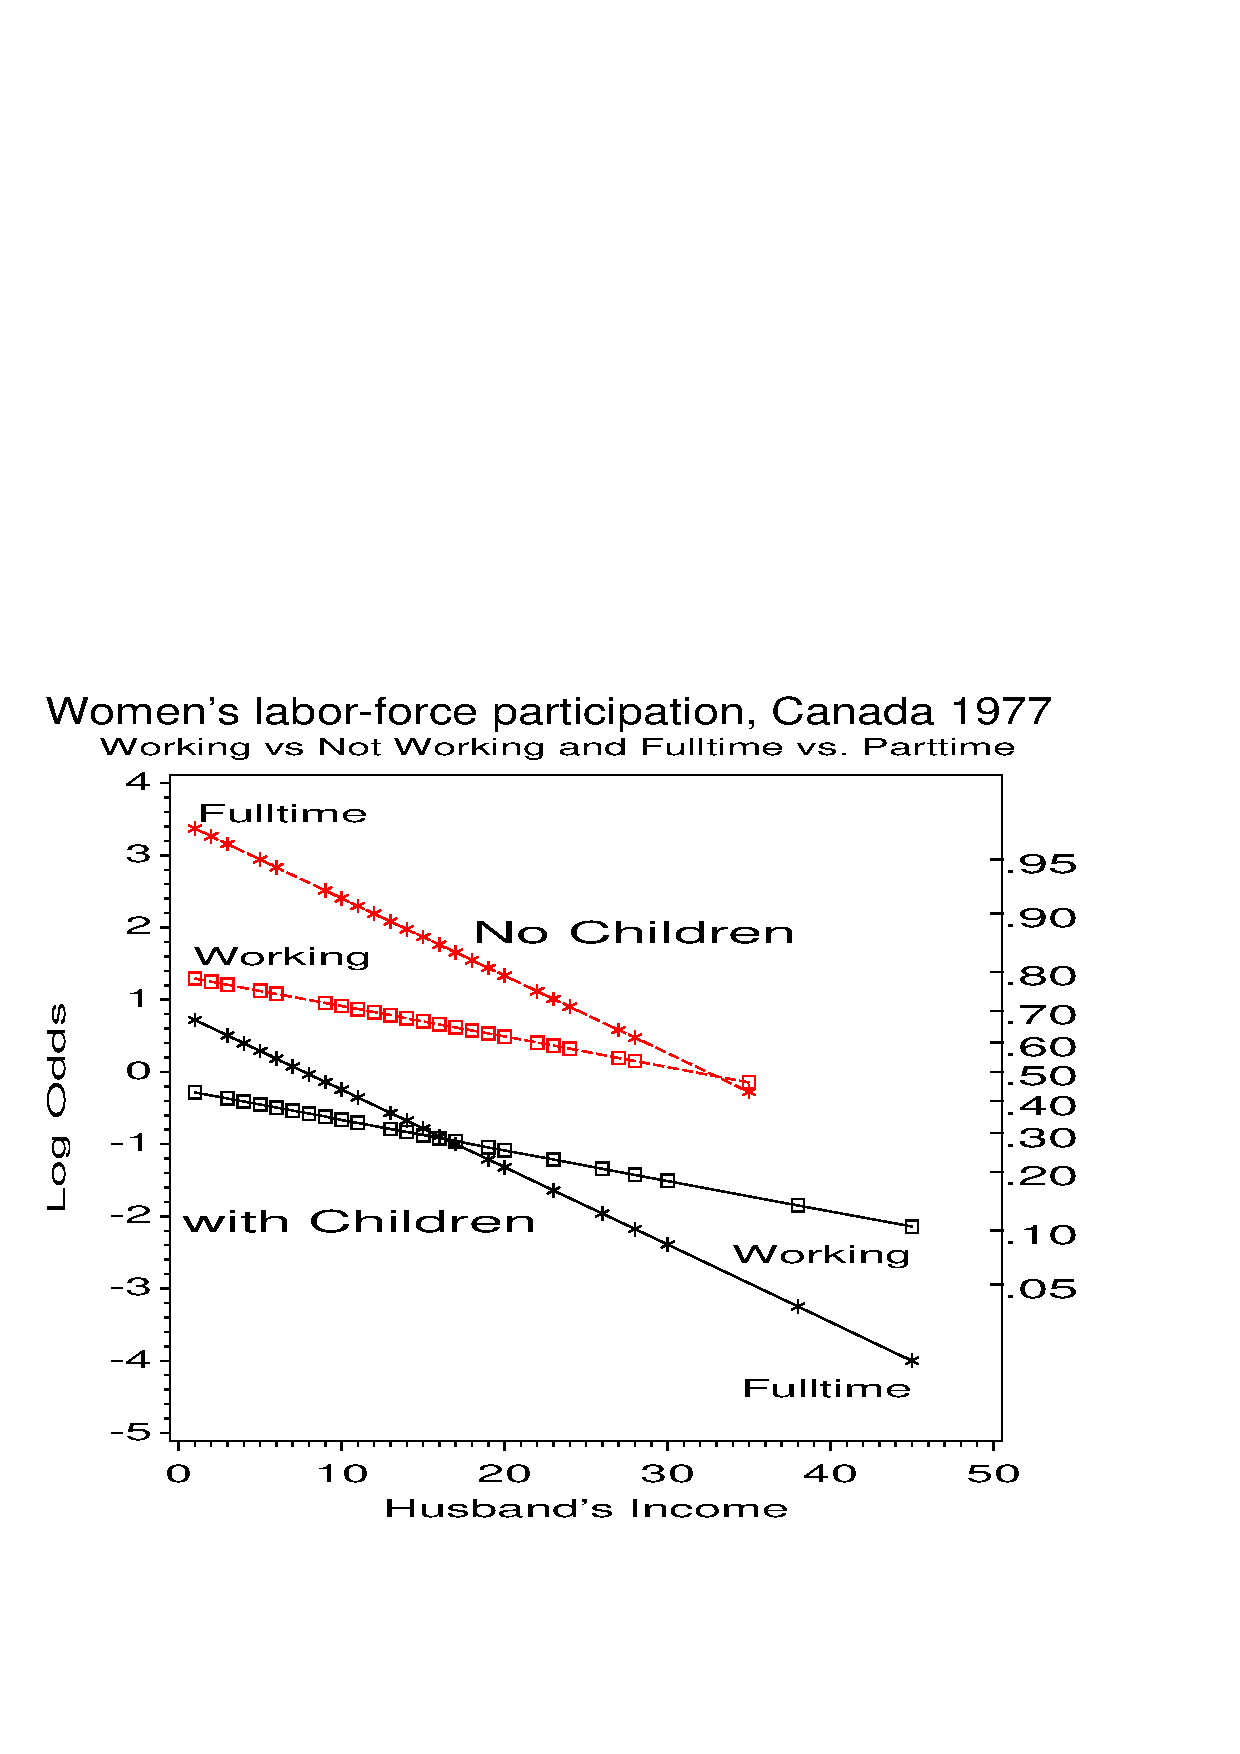
\includegraphics[height=.7\textheight]{fig/wlfpart}
\end{center}
\end{frame}

\begin{frame}[fragile]
  \frametitle{Model visualization}
  \begin{itemize*}
	\item Join \ODS{}s (\texttt{resultsw} and \texttt{resultsf})
	\item Combine Response \& Children $\rightarrow$ \texttt{event}
  \end{itemize*}
\begin{Input}
\sascomment{*-- Join the results datasets to create one plot;}
data both;
   set resultw(in=inw)     \sascomment{/* working  */}
       resultf(in=inf);    \sascomment{/* fulltime */}
   if inw then do;
      if children=1 then event='Working, with Children ';
      else event='Working, no Children ';
   end;
   else do;
      if children=1 then event='Fulltime, with Children ';
      else event='Fulltime, no Children ';
  end;
\end{Input}
\end{frame}

\begin{frame}[fragile]
  \frametitle{Model visualization}
\begin{comment}
  \begin{itemize*}
	\item \texttt{plot logit * husinc = event;} $\rightarrow$ separate lines
  \end{itemize*}
\end{comment}
\begin{Input}[baselinestretch=0.7]
proc gplot data=both;
   plot \sasemph{logit * husinc = event} /
        anno=lbl nolegend frame vaxis=axis1;
   axis1 label=(a=90 'Log Odds') order=(-5 to 4);
   title2 'Working vs Not Working and Fulltime vs. Parttime';
   symbol1 v=dot    h=1.5 i=join l=3 c=red;
   symbol2 v=dot    h=1.5 i=join l=1 c=black;
   symbol3 v=circle h=1.5 i=join l=3 c=red;
   symbol4 v=circle h=1.5 i=join l=1 c=black;
\end{Input}
\begin{center}
  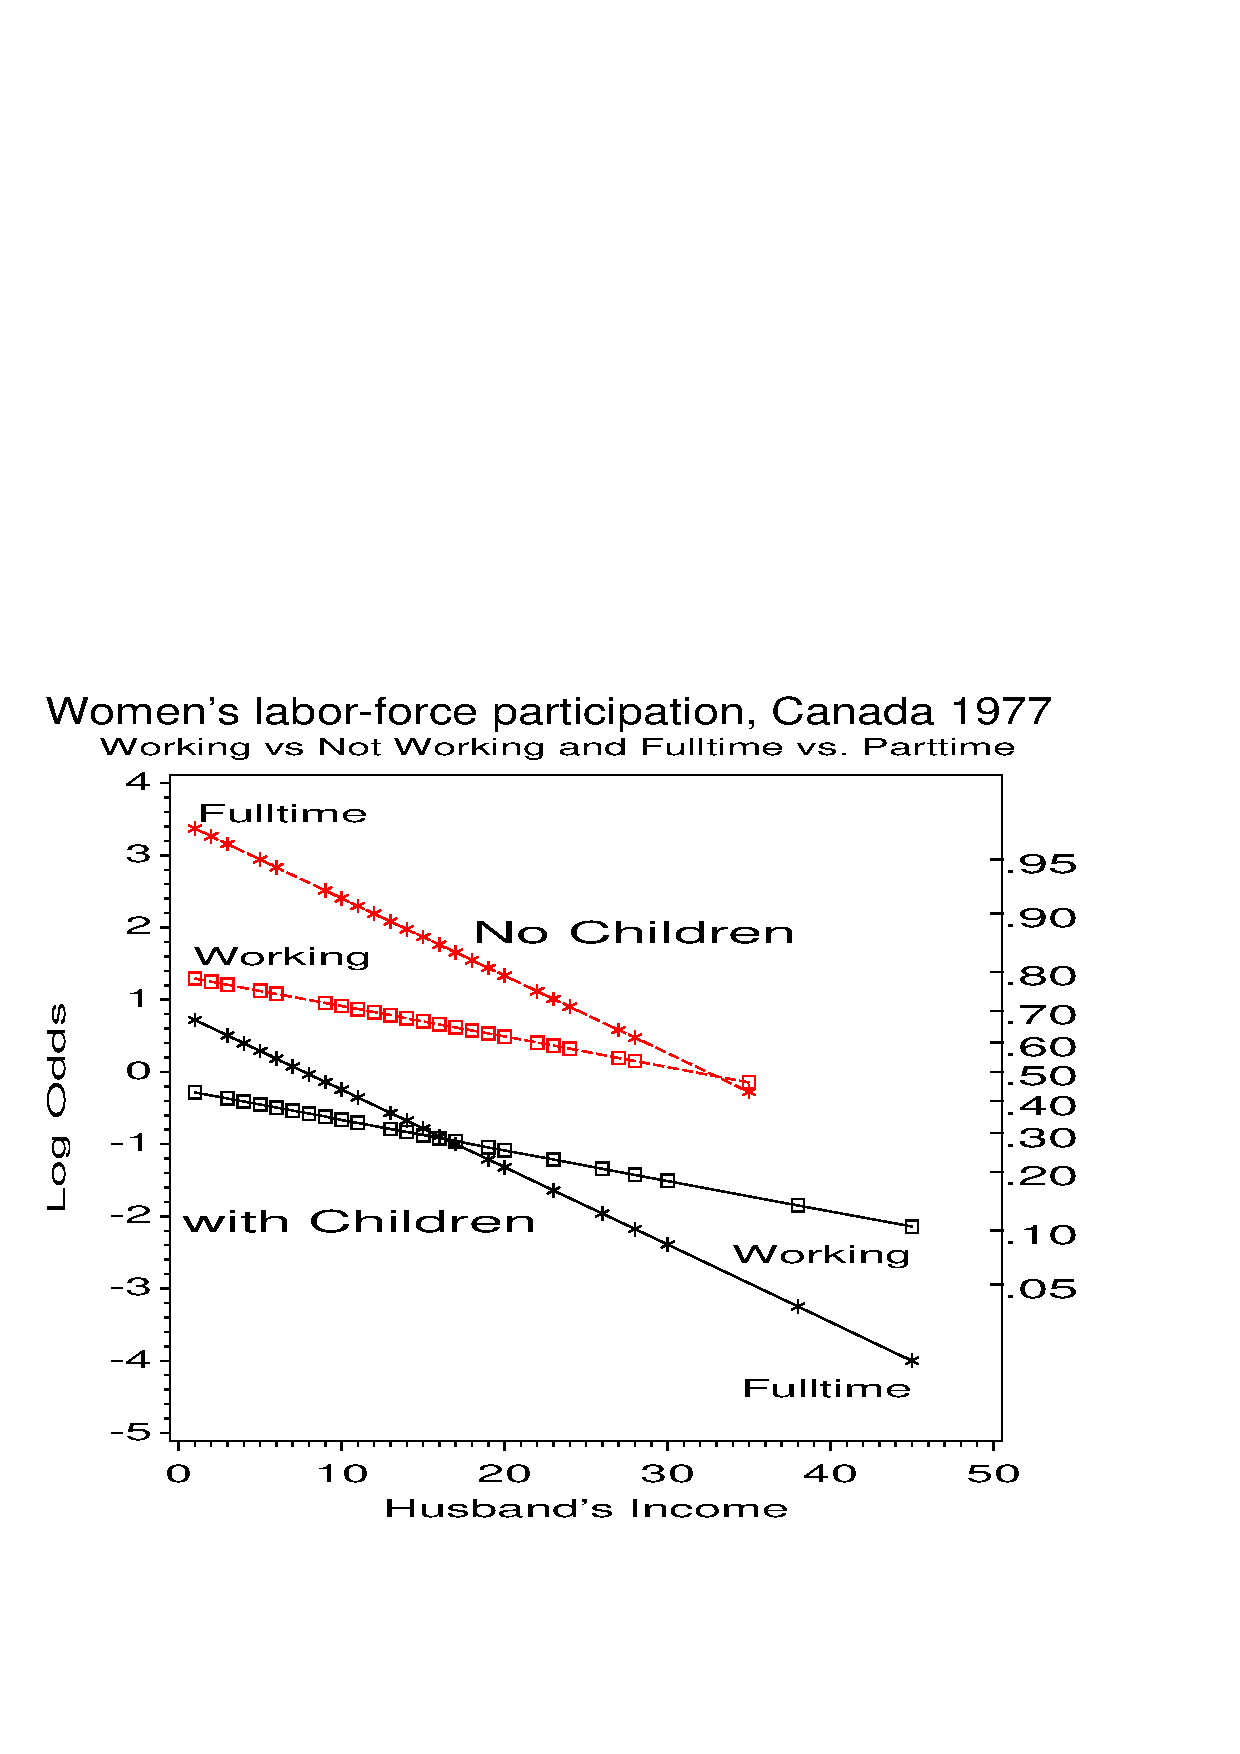
\includegraphics[height=.55\textheight]{fig/wlfpart}
\end{center}
\end{frame}

\endinput

% slide template
\begin{frame}
  \frametitle{}
  \begin{itemize}
	\item{\large\bfseries }
      \begin{itemize*}
	  \item 
    	\begin{itemize*}
		\item 
		\item 
		\end{itemize*}
	  \item 
	  \end{itemize*}
	\item{\large\bfseries }
	\item{\large\bfseries }
  \end{itemize}
\end{frame}

